\documentclass[journal]{IEEEtran}
\usepackage[a5paper,margin=10mm]{geometry}
\setlength{\headheight}{1cm}
\setlength{\headsep}{0mm}

% Keep the GVV support packages used by the reference repository in the source tree.
\usepackage{gvv-book}
\let\savedvec\vec
\usepackage{gvv}
\let\vec\savedvec

% Project-specific typesetting and the existing solution notation.
\usepackage[center]{caption}
\raggedbottom
\hypersetup{colorlinks=true,urlcolor=black,linkcolor=black,citecolor=black,hypertexnames=false,pdftitle={CBSE Class 10 Mathematics 2015}}
\makeindex

% Preserve this project's original matrix brackets and solution label.
\renewcommand{\myvec}[1]{\ensuremath{\begin{bmatrix}#1\end{bmatrix}}}
\renewcommand{\mydet}[1]{\ensuremath{\begin{vmatrix}#1\end{vmatrix}}}
\renewcommand{\solution}{\par\smallskip\noindent\textbf{Solution.}\;}
\newcounter{qcurrent}
\let\oldEqref\eqref
\renewcommand{\eqref}[1]{\textcolor{red}{\oldEqref{#1}}}

\begin{document}
\bibliographystyle{IEEEtran}
\onecolumn

\title{
  \begin{center}
  {\LARGE\bfseries Math for EE}\\
  \rule{0.4\columnwidth}{0.4pt}
  \end{center}
}
\author{
  \vspace{11cm}
  \begin{center}
  {\fontsize{26}{31}\selectfont\bfseries CBSE Class 10 2015}
  \end{center}
}
\maketitle
\thispagestyle{empty}
\newpage
\tableofcontents
\newpage

\section{Formulae}
% Formulae are numbered hierarchically and referenced by labels from solutions.
\renewcommand{\theequation}{1.1.\arabic{qcurrent}.\arabic{equation}}
\setcounter{equation}{0}

\paragraph*{Quadratic equations}
For $ax^2+bx+c=0$, where $a\ne0$, the discriminant and roots are
\setcounter{qcurrent}{1}\setcounter{equation}{0}
\par\noindent\textbf{1.1.1}\quad
\begin{equation}
\Delta=b^2-4ac,\qquad x=\frac{-b\pm\sqrt{\Delta}}{2a}.
\label{eq:quad-general}
\end{equation}
Equal real roots occur when $\Delta=0$. Always check that the leading coefficient is nonzero before treating an expression as a quadratic equation.

\paragraph*{Right-triangle trigonometry and motion}
For an angle $\theta$ in a right triangle,
\setcounter{qcurrent}{2}\setcounter{equation}{0}
\par\noindent\textbf{1.1.2}\quad
\begin{equation}
\tan\theta=\frac{\text{opposite}}{\text{adjacent}},\quad
\sin\theta=\frac{\text{opposite}}{\text{hypotenuse}},\quad
\cos\theta=\frac{\text{adjacent}}{\text{hypotenuse}}.
\label{eq:trig-ratios}
\end{equation}
Useful values are $\tan30^\circ=1/\sqrt3$, $\tan60^\circ=\sqrt3$, $\cot30^\circ=\sqrt3$, $\cot60^\circ=1/\sqrt3$, $\sin30^\circ=1/2$, and $\cos60^\circ=1/2$. For a right triangle,
\[c^2=a^2+b^2,\qquad \|(x,y)^T\|=\sqrt{x^2+y^2}.\]
Uniform motion obeys
\setcounter{qcurrent}{13}\setcounter{equation}{0}
\par\noindent\textbf{1.1.13}\quad
\begin{equation}
\text{distance}=\text{speed}\times\text{time},\qquad
\text{average speed}=\frac{\text{total distance}}{\text{total time}}.
\label{eq:speed-time}
\end{equation}
For an object at fixed height $h$ observed from level ground, its horizontal range is $x=h\cot\theta$.
In this situation,
\par\noindent\textbf{1.1.27}\quad
\begin{equation}
x=h\cot\theta.\tag{1.1.27.1}\label{eq:horizontal-range}
\end{equation}
For two parts of a journey, total time is
\par\noindent\textbf{1.1.23}\quad
\begin{equation}
t_1+t_2=\frac{d_1}{v_1}+\frac{d_2}{v_2}.\tag{1.1.23.1}\label{eq:two-part-time}
\end{equation}

\paragraph*{Probability}
For equally likely outcomes,
\setcounter{qcurrent}{3}\setcounter{equation}{0}
\par\noindent\textbf{1.1.3}\quad
\begin{equation}
P(E)=\frac{n(E)}{n(S)}.
\label{eq:prob-classical}
\end{equation}
For events $A$ and $B$,
\setcounter{qcurrent}{28}\setcounter{equation}{0}
\par\noindent\textbf{1.1.28}\quad
\begin{equation}
P(A\cup B)=P(A)+P(B)-P(A\cap B),\qquad P(A^c)=1-P(A).
\label{eq:prob-union}
\end{equation}
When two different dice are tossed, there are $6\cdot6=36$ equally likely ordered outcomes; exchanging the dice generally gives a different outcome.
If $E_1,E_2,E_3$ form an exhaustive set of mutually exclusive events, then
\par\noindent\textbf{1.1.15}\quad
\begin{equation}
P(E_1)+P(E_2)+P(E_3)=1.\tag{1.1.15.1}\label{eq:three-events}
\end{equation}

\paragraph*{Circles and tangents}
A radius is perpendicular to the tangent at the point of contact. Tangents drawn from the same external point have equal lengths. The angle between a tangent and a chord equals the angle in the alternate segment; the angle at the centre is twice the angle at the circumference standing on the same arc. For a triangle with inradius $r$ and semiperimeter $s$,
\setcounter{qcurrent}{6}\setcounter{equation}{0}
\par\noindent\textbf{1.1.6}\quad
\begin{equation}
[ABC]=rs,\qquad s=\frac{AB+BC+CA}{2}.
\label{eq:triangle-inradius}
\end{equation}
Tangents from the same external point have equal lengths:
\begin{equation}
PA=PB.\tag{1.1.6.2}\label{eq:equal-tangents}
\end{equation}
The tangent--chord theorem is
\par\noindent\textbf{1.1.4}\quad
\begin{equation}
\theta_{\mathrm{tangent-chord}}=\theta_{\mathrm{alternate\ segment}}.\tag{1.1.4.1}\label{eq:tangent-chord}
\end{equation}

\paragraph*{Arithmetic progressions}
For first term $a$ and common difference $d$,
\setcounter{qcurrent}{8}\setcounter{equation}{0}
\par\noindent\textbf{1.1.8}\quad
\begin{equation}
t_n=a+(n-1)d,\qquad
S_n=\frac n2\bigl(2a+(n-1)d\bigr)=\frac n2(a+t_n).
\label{eq:ap}
\end{equation}
If the unknown parameters satisfy two linear equations, write them as an augmented matrix and use Gaussian elimination (elementary row operations) to solve the system.
For an arithmetic progression,
\par\noindent\textbf{1.1.11}\quad
\begin{equation}
 t_n=a+(n-1)d,\qquad S_n=\frac n2\left(2a+(n-1)d\right).\tag{1.1.11.1}\label{eq:ap-question-11}
\end{equation}
The sum of terms $m$ through $n$ is
\par\noindent\textbf{1.1.22}\quad
\begin{equation}
S_{m\ldots n}=S_n-S_{m-1}.\tag{1.1.22.1}\label{eq:ap-subsum}
\end{equation}

\paragraph*{Coordinate geometry as linear algebra}
Represent $P(x,y)$ by $\vec p=\myvec{x\\y}$. Then
\setcounter{qcurrent}{14}\setcounter{equation}{0}
\par\noindent\textbf{1.1.14}\quad
\begin{equation}
\overrightarrow{PQ}=\vec q-\vec p,\qquad
\langle\vec u,\vec v\rangle=u_xv_x+u_yv_y.
\label{eq:vector-basics}
\end{equation}
Two nonzero vectors are perpendicular exactly when their inner product is zero.
For a right angle at $B$,
\par\noindent\textbf{1.1.9}\quad
\begin{equation}
\overrightarrow{BA}\cdot\overrightarrow{BC}=0.\tag{1.1.9.1}\label{eq:right-angle-dot}
\end{equation}
For $A(x_1,y_1)$, $B(x_2,y_2)$, and $C(x_3,y_3)$, collinearity is equivalent to
\setcounter{qcurrent}{10}\setcounter{equation}{0}
\par\noindent\textbf{1.1.10}\quad
\begin{equation}
\mydet{x_2-x_1&y_2-y_1\\x_3-x_1&y_3-y_1}=0.
\label{eq:collinear-det}
\end{equation}
The triangle area is half the absolute determinant:
\setcounter{qcurrent}{29}\setcounter{equation}{0}
\par\noindent\textbf{1.1.29}\quad
\begin{equation}
[ABC]=\frac12\left|\mydet{x_2-x_1&y_2-y_1\\x_3-x_1&y_3-y_1}\right|.
\label{eq:triangle-det}
\end{equation}
If $P$ divides $AB$ internally in the ratio $AP:PB=m:n$, then
\setcounter{qcurrent}{14}\setcounter{equation}{0}
\setcounter{qcurrent}{14}\setcounter{equation}{1}
\par\noindent\textbf{1.1.14}\quad
\begin{equation}
\vec p=\frac{n\vec a+m\vec b}{m+n}=\vec a+\frac{m}{m+n}(\vec b-\vec a).
\label{eq:section-vector}
\end{equation}
\paragraph*{Areas and solids}
For a sector of angle $\theta$ degrees and radius $r$,
\setcounter{qcurrent}{16}\setcounter{equation}{0}
\par\noindent\textbf{1.1.16}\quad
\begin{equation}
A_{\mathrm{sector}}=\frac{\theta}{360^\circ}\pi r^2,\qquad
A_{\mathrm{segment}}=A_{\mathrm{sector}}-A_{\mathrm{triangle}}.
\label{eq:sector-segment}
\end{equation}
The curved surface areas of a cylinder and a cone are
\setcounter{qcurrent}{17}\setcounter{equation}{0}
\par\noindent\textbf{1.1.17}\quad
\begin{equation}
A_{\mathrm{cyl}}=2\pi rh,\qquad A_{\mathrm{cone}}=\pi r\ell,\qquad \ell=\sqrt{r^2+h^2}.
\label{eq:cone-formula}
\end{equation}
The corresponding volume formula for a cylinder is
\setcounter{qcurrent}{31}\setcounter{equation}{0}
\par\noindent\textbf{1.1.31}\quad
\begin{equation}
V_{\mathrm{cyl}}=\pi r^2h.
\label{eq:cylinder-formula}
\end{equation}
For a hemisphere and sphere,
\setcounter{qcurrent}{31}\setcounter{equation}{0}
\setcounter{qcurrent}{31}\setcounter{equation}{1}
\begin{equation}
V_{\mathrm{hemisphere}}=\frac23\pi r^3,\qquad V_{\mathrm{sphere}}=\frac43\pi r^3,
\qquad A_{\mathrm{sphere}}=4\pi r^2.
\label{eq:sphere-formula}
\end{equation}
A shaded region between an outer and an inner shape has area
\par\noindent\textbf{1.1.30}\quad
\begin{equation}
A_{\mathrm{shaded}}=A_{\mathrm{outer}}-A_{\mathrm{inner}}.\tag{1.1.30.1}\label{eq:shaded-area}
\end{equation}
For a cylinder with two hemispherical cavities of radius $r$ scooped from its ends,
\setcounter{qcurrent}{31}\setcounter{equation}{0}
\setcounter{qcurrent}{31}\setcounter{equation}{2}
\par\noindent\textbf{1.1.31}\quad
\begin{equation}
V_{\mathrm{remaining}}=\pi R^2h-\frac43\pi r^3.
\label{eq:scooped-cylinder}
\end{equation}

\newpage
\section{Problems}
% Question labels retain the original paper numbering, even where questions were omitted.
\renewcommand{\theequation}{1.1.\arabic{qcurrent}.\arabic{equation}}

\begin{enumerate}[label={},leftmargin=0pt,itemsep=9pt]
\setcounter{qcurrent}{1}\setcounter{equation}{0}
\item[\textbf{1.2.1}] If the quadratic equation $px^2-2\sqrt5\,px+15=0$ has two equal roots, find $p$.
\solution By \eqref{eq:quad-general}, its discriminant must be zero:
\begin{align}
(-2\sqrt5p)^2-4(p)(15)&=0\\
20p^2-60p&=0\\
20p(p-3)&=0.
\end{align}
The algebra gives $p=0$ or $p=3$. The first value removes the quadratic and linear terms and leaves $15=0$, which is impossible. Therefore $p=3$.



\begin{figure}[H]\centering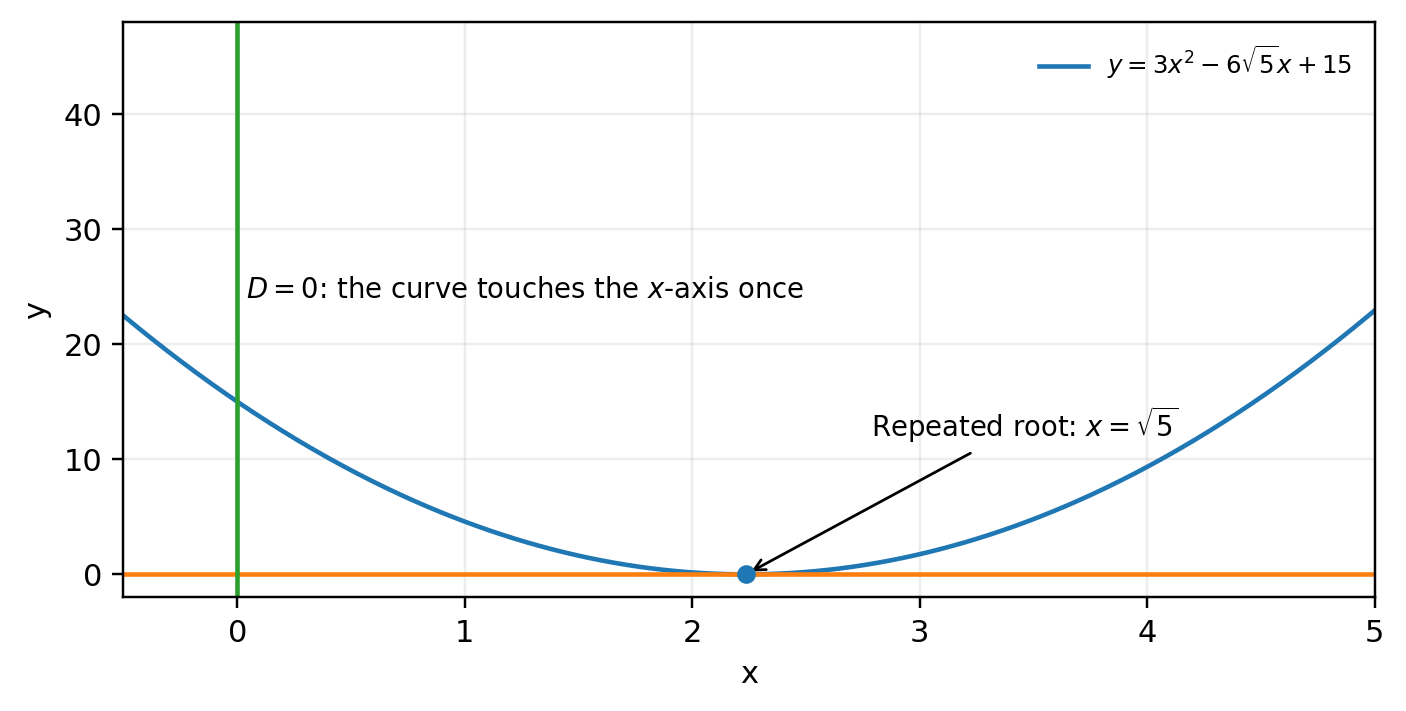
\includegraphics[width=0.92\linewidth]{figs/Q01_Quadratic.png}\caption{For $p=3$, the quadratic touches the $x$-axis at its repeated root $x=\sqrt{5}$, showing that there is only one distinct root.}\label{fig:q1-quadratic}\end{figure}
The Python code uses the theoretically derived value $p=3$ and plots its parabola:
\par\smallskip
\noindent\textbf{Code reference -- plotting}
\par\noindent\fbox{\parbox{\dimexpr\linewidth-2\fboxsep-2\fboxrule\relax}{\centering\texttt{codes/Q01.py}}}
\par\smallskip
\setcounter{qcurrent}{2}\setcounter{equation}{0}
\item[\textbf{1.2.2}] A tower $AB$ is $20\,\mathrm m$ high and its shadow $BC$ is $20\sqrt3\,\mathrm m$ long. Find the Sun's altitude.
\begin{figure}[H]\centering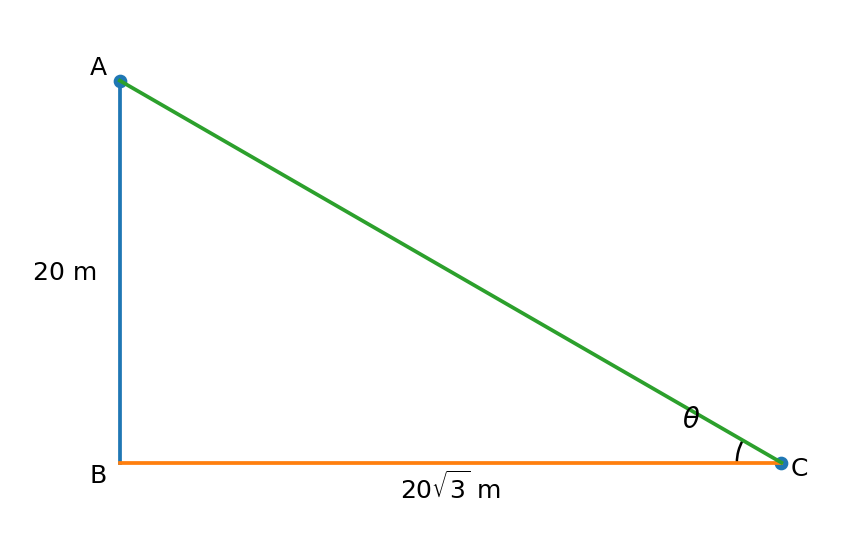
\includegraphics[width=0.78\linewidth]{figs/Tower.png}\caption{Tower and its shadow.}\label{fig:tower}\end{figure}
\solution Let the angle of elevation be $\theta$. From the right triangle and \eqref{eq:trig-ratios},
\begin{equation}
\tan\theta=\frac{AB}{BC}=\frac{20}{20\sqrt3}=\frac1{\sqrt3}.
\end{equation}
Thus $\theta=30^\circ$.



The tower-and-shadow diagram is generated by this script:
\par\smallskip
\noindent\textbf{Code reference -- plotting}
\par\noindent\fbox{\parbox{\dimexpr\linewidth-2\fboxsep-2\fboxrule\relax}{\centering\texttt{codes/Q02.py}}}
\par\smallskip
\newpage
\setcounter{qcurrent}{3}\setcounter{equation}{0}
\item[\textbf{1.2.3}] Two different dice are tossed together. Find the probability that the product of their top numbers is $6$.
\solution Each cell in the table gives the product of the ordered outcome $(\text{Die 1},\text{Die 2})$. There are $6\times6=36$ equally likely outcomes.
\begin{table}[H]\centering\small
\caption{Products for all 36 ordered dice outcomes. The four products equal to 6 are highlighted.}
\setlength{\tabcolsep}{5pt}
\begin{tabular}{c|rrrrrr}
\hline
Die 1 $\backslash$ Die 2 & 1 & 2 & 3 & 4 & 5 & 6\\\hline
1 & 1 & 2 & 3 & 4 & 5 & $\mathbf{6}$\\
2 & 2 & 4 & $\mathbf{6}$ & 8 & 10 & 12\\
3 & 3 & $\mathbf{6}$ & 9 & 12 & 15 & 18\\
4 & 4 & 8 & 12 & 16 & 20 & 24\\
5 & 5 & 10 & 15 & 20 & 25 & 30\\
6 & $\mathbf{6}$ & 12 & 18 & 24 & 30 & 36\\
\hline
\end{tabular}\end{table}
The favourable outcomes are $(1,6),(2,3),(3,2),(6,1)$, so
\begin{equation}
P(\text{product}=6)=\frac4{36}=\frac19.
\end{equation}



\begin{figure}[H]\centering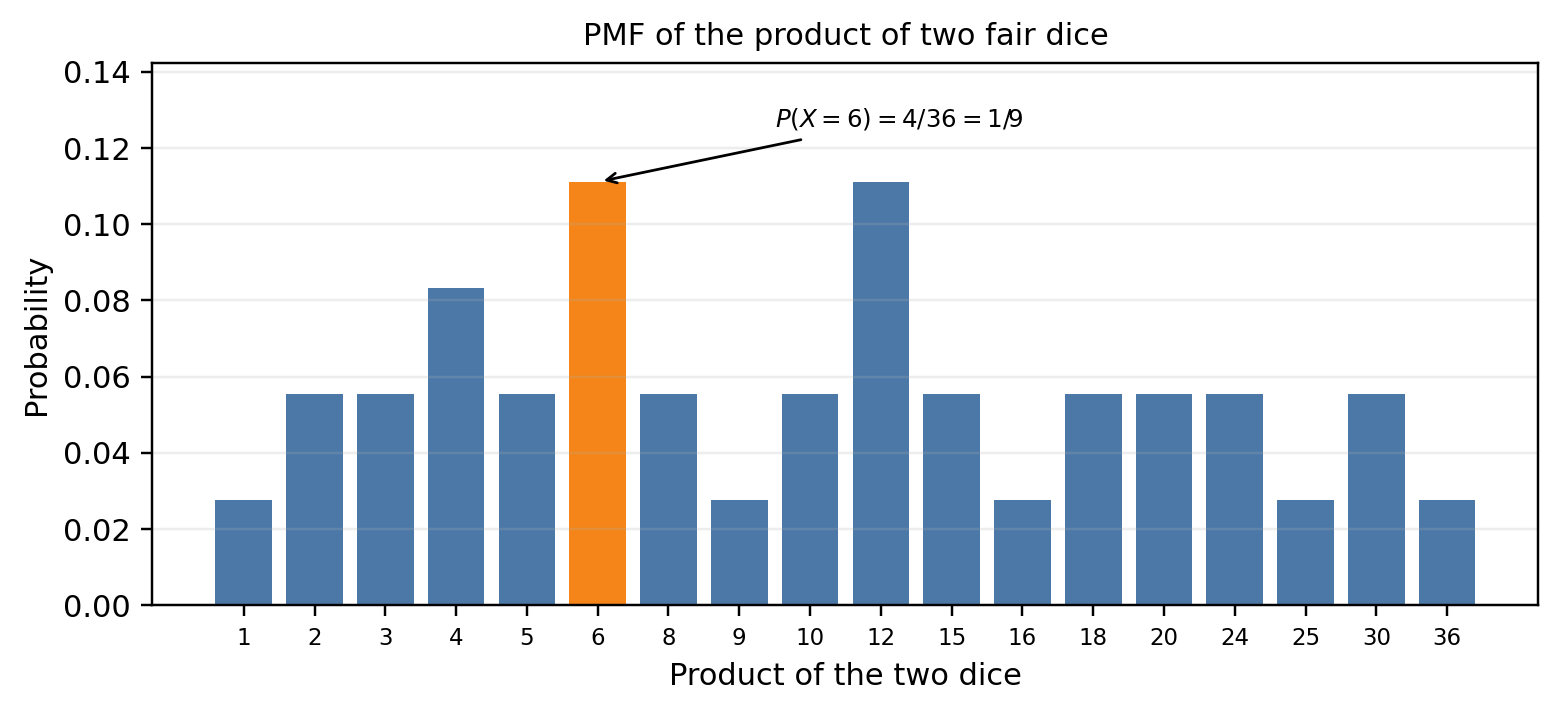
\includegraphics[width=0.98\linewidth]{figs/Q03_ProductPMF.png}\caption{Probability mass function of the product of two distinguishable fair dice. The bar at 6 represents the four favourable ordered outcomes.}\label{fig:q3-pmf}\end{figure}
The Python code uses the theoretically counted favourable outcomes for each product, divides each count by 36, and plots the probability mass function:
\par\smallskip
\noindent\textbf{Code reference -- plotting}
\par\noindent\fbox{\parbox{\dimexpr\linewidth-2\fboxsep-2\fboxrule\relax}{\centering\texttt{codes/Q03.py}}}
\par\smallskip
\newpage
\setcounter{qcurrent}{4}\setcounter{equation}{0}
\item[\textbf{1.2.4}] $PQ$ is a chord of a circle with centre $O$, and $PT$ is a tangent. If $\angle QPT=60^\circ$, find $\angle PRQ$.
\begin{figure}[H]\centering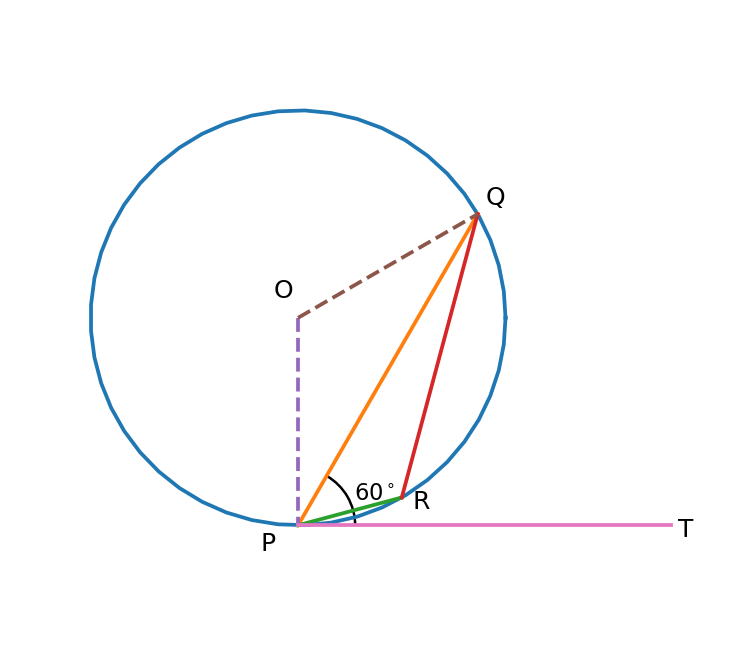
\includegraphics[width=0.72\linewidth]{figs/TangentChord.png}\caption{Chord--tangent configuration.}\label{fig:tangent-chord}\end{figure}
\solution Since $OP\perp PT$, we have $\angle OPQ=30^\circ$. As $OP=OQ$, triangle $OPQ$ is isosceles, so $\angle OQP=30^\circ$ and $\angle POQ=120^\circ$. With $R$ on the minor arc $PQ$, the intercepted major arc measures $240^\circ$. An angle at the circumference is half its intercepted arc, hence $\angle PRQ=120^\circ$.


The circle-and-tangent diagram is generated by this script:
\par\smallskip
\noindent\textbf{Code reference -- plotting}
\par\noindent\fbox{\parbox{\dimexpr\linewidth-2\fboxsep-2\fboxrule\relax}{\centering\texttt{codes/Q04.py}}}
\par\smallskip
\end{enumerate}

\newpage
\begin{enumerate}[label={},leftmargin=0pt,itemsep=9pt]
\setcounter{qcurrent}{6}\setcounter{equation}{0}
\item[\textbf{1.2.6}] A triangle circumscribes a circle of radius $3\,\mathrm{cm}$. The base portions are $BD=6\,\mathrm{cm}$ and $DC=9\,\mathrm{cm}$. If the triangle's area is $54\,\mathrm{cm}^2$, find $AB$ and $AC$.
\begin{figure}[H]\centering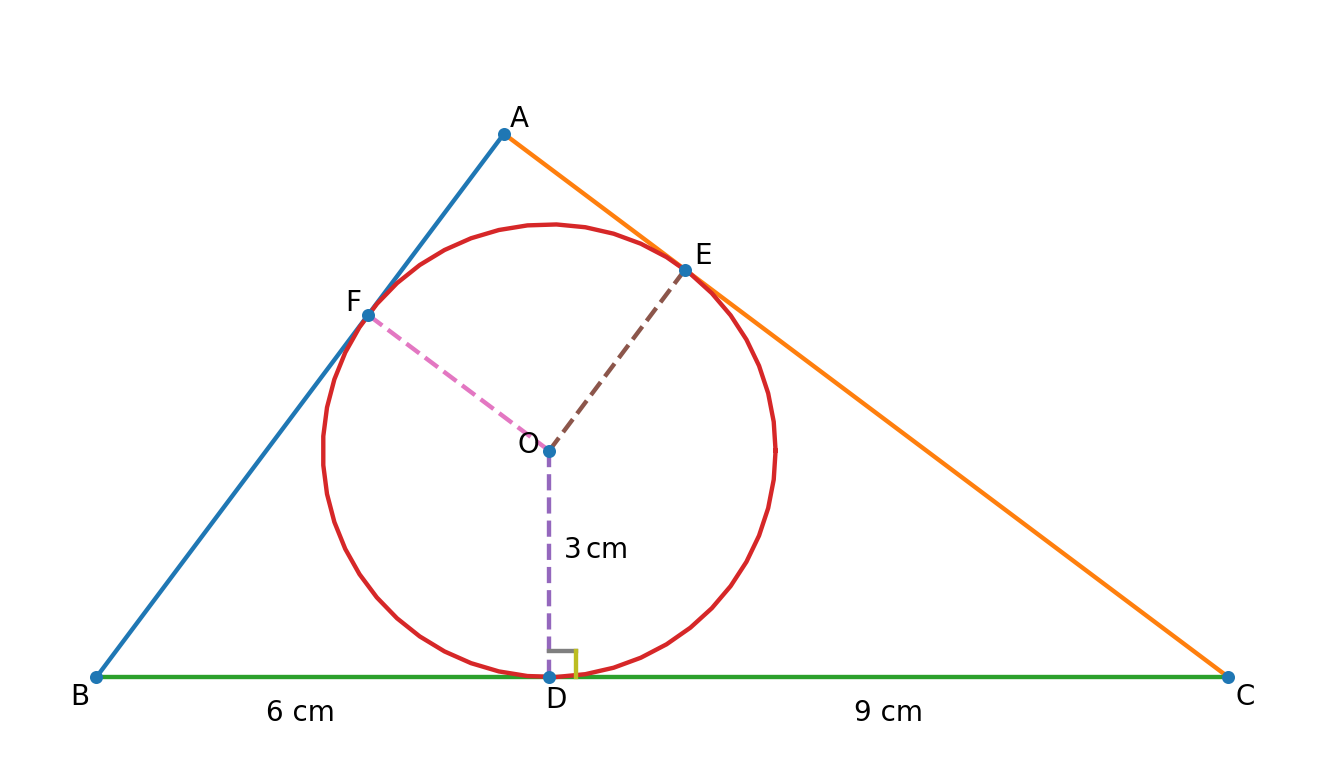
\includegraphics[width=0.78\linewidth]{figs/IncircleTriangle.png}\caption{Triangle with an incircle.}\label{fig:incircle}\end{figure}
\solution By \eqref{eq:triangle-inradius}, the semiperimeter is
\begin{equation}
s=\frac{[ABC]}r=\frac{54}{3}=18\,\mathrm{cm}.
\end{equation}
Tangents from a common external point have equal lengths. Let the tangent length from $A$ be $x$. Then $AB=x+6$, $AC=x+9$, and $BC=15$. Consequently,
\begin{equation}
s=\frac{(x+6)+(x+9)+15}{2}=x+15=18,
\end{equation}
so $x=3$. Therefore $AB=9\,\mathrm{cm},\quad AC=12\,\mathrm{cm}$.



The incircle diagram is generated by this script:
\par\smallskip
\noindent\textbf{Code reference -- plotting}
\par\noindent\fbox{\parbox{\dimexpr\linewidth-2\fboxsep-2\fboxrule\relax}{\centering\texttt{codes/Q06.py}}}
\par\smallskip
\newpage
\setcounter{qcurrent}{8}\setcounter{equation}{0}
\item[\textbf{1.2.8}] In an arithmetic progression, $S_5+S_7=167$ and $S_{10}=235$. Find the AP.
\solution Let the first term be $a$ and the common difference be $d$. By \eqref{eq:ap},
\begin{align}
S_5&=5a+10d, & S_7&=7a+21d, & S_{10}&=10a+45d.
\end{align}
The conditions therefore give the linear system
\begin{equation}
\myvec{12&31\\10&45}\myvec{a\\d}=\myvec{167\\235}.
\label{eq:q8system}
\end{equation}
Apply Gaussian elimination to the augmented matrix:
\begin{equation}
\left[\begin{array}{cc|c}12&31&167\\10&45&235\end{array}\right]
\xrightarrow{\;R_2\leftarrow6R_2-5R_1\;}
\left[\begin{array}{cc|c}12&31&167\\0&115&575\end{array}\right].
\end{equation}
The second row gives $115d=575$, so $d=5$. Substituting this into the first row gives $12a+31(5)=167$, hence $a=1$. The AP is $1,6,11,16,\ldots$.



This script uses NumPy's linear solver to compare the theoretical values with the solution of the two-equation system:
\par\smallskip
\noindent\textbf{Code reference -- numerical verification}
\par\noindent\fbox{\parbox{\dimexpr\linewidth-2\fboxsep-2\fboxrule\relax}{\centering\texttt{codes/Q08.py}}}
\par\smallskip
\setcounter{qcurrent}{9}\setcounter{equation}{0}
\item[\textbf{1.2.9}] $A(4,7)$, $B(p,3)$ and $C(7,3)$ form a right triangle, right-angled at $B$. Find $p$.
\solution The two side vectors meeting at $B$ are
\begin{equation}
\overrightarrow{BA}=\myvec{4-p\\4},\qquad \overrightarrow{BC}=\myvec{7-p\\0}.
\end{equation}
Since the sides are perpendicular, their inner product is zero by \eqref{eq:vector-basics}:
\begin{equation}
\langle\overrightarrow{BA},\overrightarrow{BC}\rangle=(4-p)(7-p)=0.
\end{equation}
Thus $p=4$ or $p=7$. The second value makes $B=C$, so it does not form a triangle. Hence $p=4$.




\setcounter{qcurrent}{10}\setcounter{equation}{0}
\item[\textbf{1.2.10}] If $A(x,y)$, $B(-5,7)$ and $C(-4,5)$ are collinear, find the relation between $x$ and $y$.
\solution By the determinant criterion in \eqref{eq:collinear-det},
\begin{equation}
\mydet{x+5&y-7\\1&-2}=0.
\end{equation}
Expanding gives $-2(x+5)-(y-7)=0$, and hence $2x+y+3=0$.



\end{enumerate}

\newpage
\begin{enumerate}[label={},leftmargin=0pt,itemsep=9pt]
\setcounter{qcurrent}{11}\setcounter{equation}{0}
\item[\textbf{1.2.11}] The 14th term of an AP is twice its 8th term. If the 6th term is $-8$, find the sum of its first 20 terms.
\solution Let $a$ and $d$ denote the first term and common difference. The first condition is
\begin{equation}
a+13d=2(a+7d)\quad\Longrightarrow\quad a+d=0.
\end{equation}
The sixth-term condition gives $a+5d=-8$. With $a=-d$, we obtain $4d=-8$, so $d=-2$ and $a=2$. Therefore
\begin{equation}
S_{20}=\frac{20}{2}\bigl(2(2)+19(-2)\bigr)=-340.
\end{equation}



The AP terms and sum are checked by this script:
\par\smallskip
\noindent\textbf{Code reference -- numerical verification}
\par\noindent\fbox{\parbox{\dimexpr\linewidth-2\fboxsep-2\fboxrule\relax}{\centering\texttt{codes/Q11.py}}}
\par\smallskip
\setcounter{qcurrent}{13}\setcounter{equation}{0}
\item[\textbf{1.2.13}] An aeroplane is observed at an elevation of $60^\circ$ from point $A$. After 15 seconds, the elevation becomes $30^\circ$. If its altitude remains $1500\sqrt3\,\mathrm m$, find its speed in km/h.
\begin{figure}[H]\centering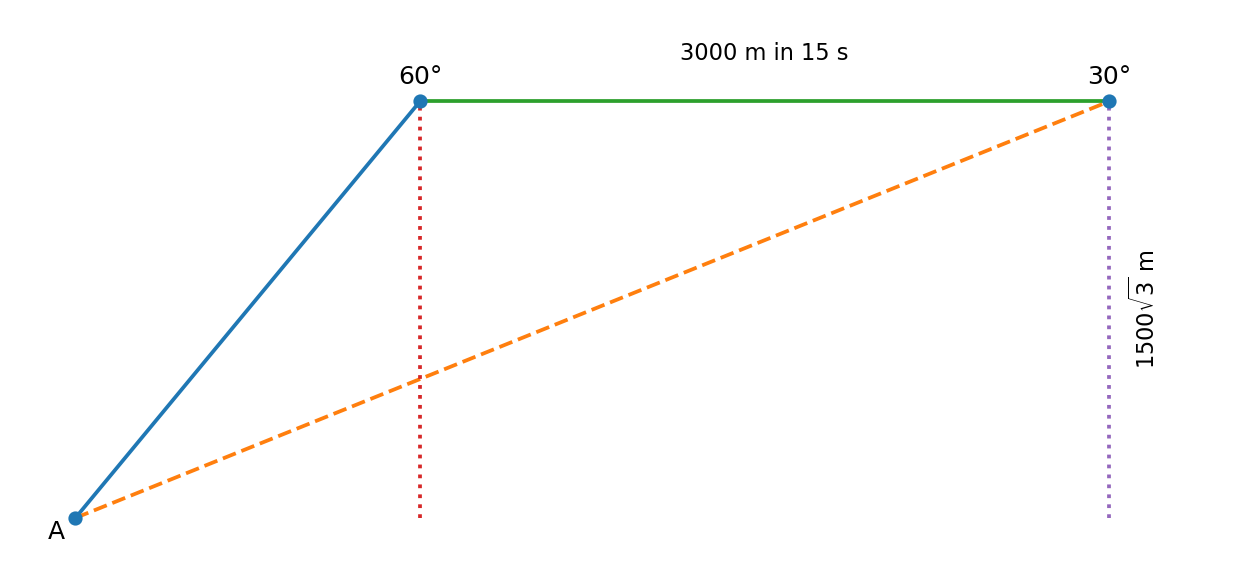
\includegraphics[width=0.86\linewidth]{figs/Aeroplane.png}\caption{The plane moves horizontally while staying at the same altitude.}\label{fig:aeroplane}\end{figure}
\solution Let its initial and final horizontal ranges be $x_1$ and $x_2$. Since the altitude $h$ is fixed, $x=h\cot\theta$:
\begin{align}
x_1&=1500\sqrt3\cot60^\circ=1500\,\mathrm m,\\
x_2&=1500\sqrt3\cot30^\circ=4500\,\mathrm m.
\end{align}
The plane covers $x_2-x_1=3000\,\mathrm m$ in 15 s. Therefore, by \eqref{eq:speed-time},
\begin{equation}
v=\frac{3000}{15}=200\,\mathrm{m/s}=200\times\frac{18}{5}=720\,\mathrm{km/h}.
\end{equation}



The speed calculation and accompanying figure are generated by this script:
\par\smallskip
\noindent\textbf{Code reference -- plotting}
\par\noindent\fbox{\parbox{\dimexpr\linewidth-2\fboxsep-2\fboxrule\relax}{\centering\texttt{codes/Q13.py}}}
\par\smallskip
\newpage
\setcounter{qcurrent}{14}\setcounter{equation}{0}
\item[\textbf{1.2.14}] $A(-2,-2)$ and $B(2,-4)$. Find the point $P$ on segment $AB$ for which $AP=\frac37 AB$.
\begin{figure}[H]\centering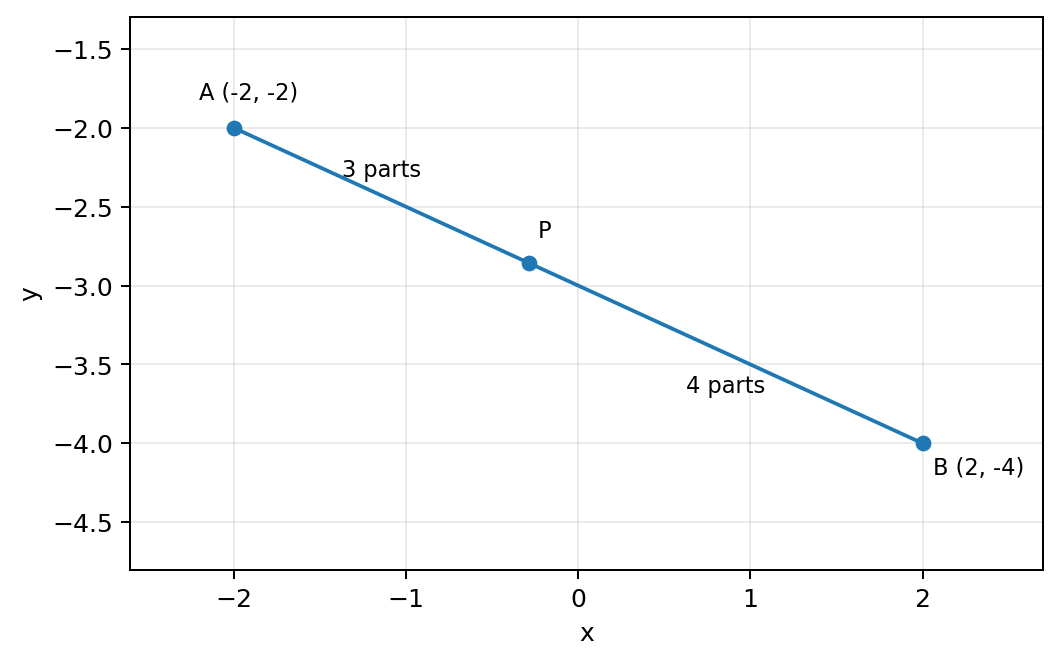
\includegraphics[width=0.82\linewidth]{figs/SectionPoint.png}\caption{The point $P$ is three-sevenths of the way from $A$ to $B$.}\label{fig:section-point}\end{figure}
\solution The section formula \eqref{eq:section-vector} gives
\begin{align}
\vec p&=\vec a+\frac37(\vec b-\vec a)\\
&=\myvec{-2\\-2}+\frac37\myvec{4\\-2}=\myvec{-2/7\\-20/7}.
\end{align}
Hence $P\left(-\frac27,-\frac{20}{7}\right)$.



The section-formula diagram is generated by this script:
\par\smallskip
\noindent\textbf{Code reference -- plotting}
\par\noindent\fbox{\parbox{\dimexpr\linewidth-2\fboxsep-2\fboxrule\relax}{\centering\texttt{codes/Q14.py}}}
\par\smallskip
\setcounter{qcurrent}{15}\setcounter{equation}{0}
\item[\textbf{1.2.15}] A jar contains only red, blue and orange balls. The probabilities of drawing a red and a blue ball are $\frac14$ and $\frac13$, respectively. If there are 10 orange balls, find the total number of balls.
\solution Let $N$ be the total number of balls. Write each probability separately:
\begin{align}
P(R)&=\frac{\text{number of red balls}}{N}=\frac14,\\
P(B)&=\frac{\text{number of blue balls}}{N}=\frac13,\\
P(O)&=\frac{\text{number of orange balls}}{N}=\frac{10}{N}.
\end{align}
Since every ball is one of these three colours, $P(R)+P(B)+P(O)=1$. Thus
\begin{equation}
\frac14+\frac13+\frac{10}{N}=1\quad\Longrightarrow\quad\frac{10}{N}=\frac5{12}\quad\Longrightarrow\quad N=24.
\end{equation}
So there are $24$ balls in total: 6 red, 8 blue and 10 orange.



\begin{figure}[H]\centering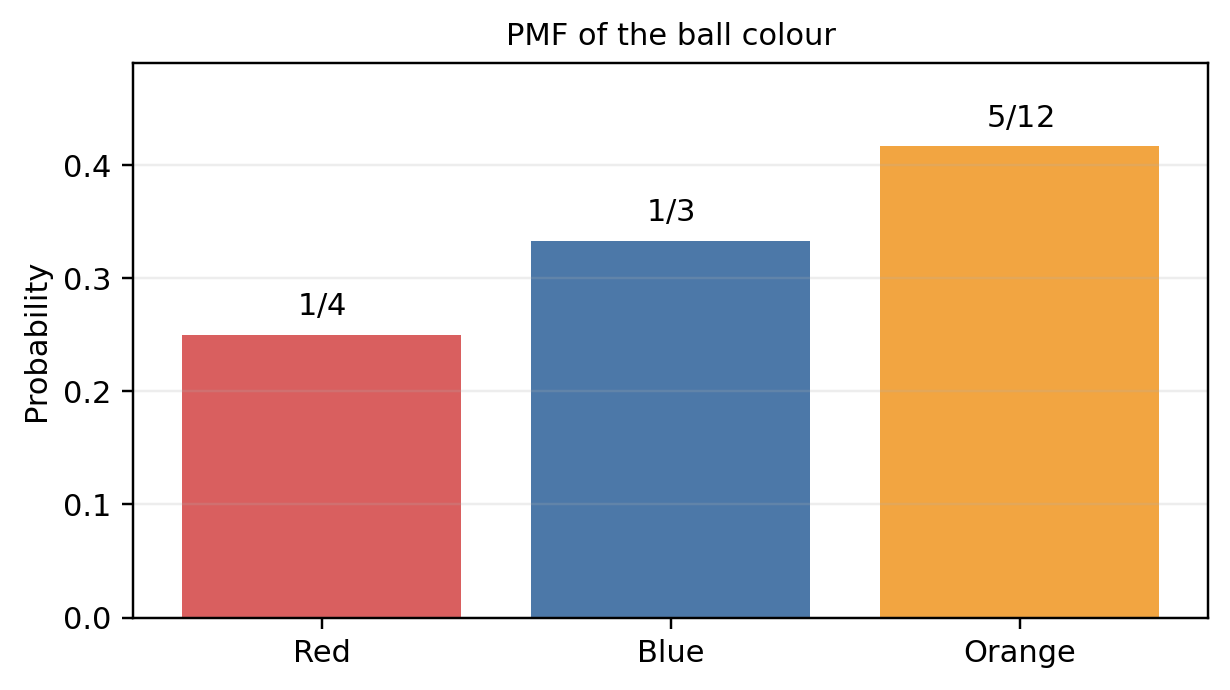
\includegraphics[width=0.9\linewidth]{figs/Q15_ColourPMF.png}\caption{Probability mass function for drawing each ball colour. The three probabilities sum to 1.}\label{fig:q15-pmf}\end{figure}
The Python code plots the theoretically derived probabilities $1/4$, $1/3$, and $5/12$ as a probability mass function:
\par\smallskip
\noindent\textbf{Code reference -- plotting}
\par\noindent\fbox{\parbox{\dimexpr\linewidth-2\fboxsep-2\fboxrule\relax}{\centering\texttt{codes/Q15.py}}}
\par\smallskip
\newpage
\setcounter{qcurrent}{16}\setcounter{equation}{0}
\item[\textbf{1.2.16}] Find the minor and major segment areas of a circle of radius $14\,\mathrm{cm}$ cut by a chord subtending $60^\circ$ at the centre. Use $\pi=\frac{22}{7}$.
\begin{figure}[H]\centering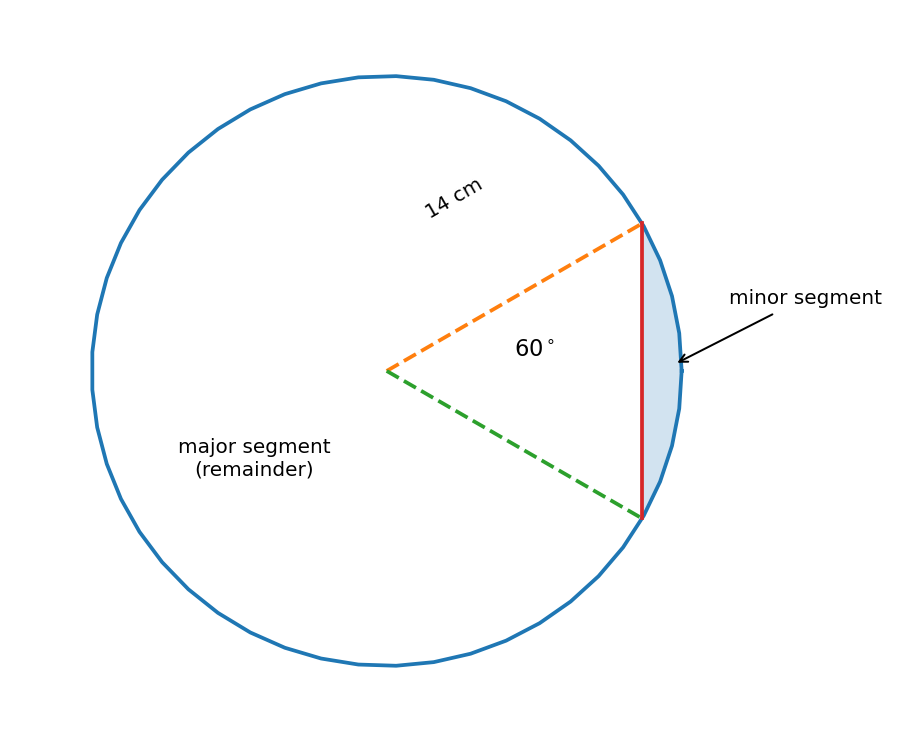
\includegraphics[width=0.86\linewidth]{figs/SegmentAreas.png}\caption{The minor segment is the small cap; the major segment is the remainder of the circle.}\label{fig:segment-areas}\end{figure}
\solution The sector angle is $60^\circ$, so \eqref{eq:sector-segment} gives
\begin{equation}
A_{\mathrm{sector}}=\frac{60}{360}\pi(14)^2=\frac{308}{3}\,\mathrm{cm}^2.
\end{equation}
The triangle between the two radii has two sides 14 cm and included angle $60^\circ$, so it is equilateral. Its area is $\frac{\sqrt3}{4}(14)^2=49\sqrt3\,\mathrm{cm}^2$. Subtracting this triangle from the sector gives
\begin{equation}
A_{\mathrm{minor}}=\frac{308}{3}-49\sqrt3\,\mathrm{cm}^2.
\end{equation}
The whole circle has area $\pi(14)^2=616\,\mathrm{cm}^2$. Therefore
\begin{equation}
A_{\mathrm{major}}=616-A_{\mathrm{minor}}=\frac{1540}{3}+49\sqrt3\,\mathrm{cm}^2.
\end{equation}



The segment diagram and area check are generated by this script:
\par\smallskip
\noindent\textbf{Code reference -- plotting}
\par\noindent\fbox{\parbox{\dimexpr\linewidth-2\fboxsep-2\fboxrule\relax}{\centering\texttt{codes/Q16.py}}}
\par\smallskip
\newpage
\setcounter{qcurrent}{17}\setcounter{equation}{0}
\item[\textbf{1.2.17}] One tent has a cylindrical lower part of diameter $4.2\,\mathrm m$ and height $4\,\mathrm m$, topped by a cone with the same diameter and height $2.8\,\mathrm m$. Canvas costs Rs. 100 per $\mathrm m^2$. Find the associations' 50\% contribution for 100 tents, and state the values shown.
\begin{figure}[H]\centering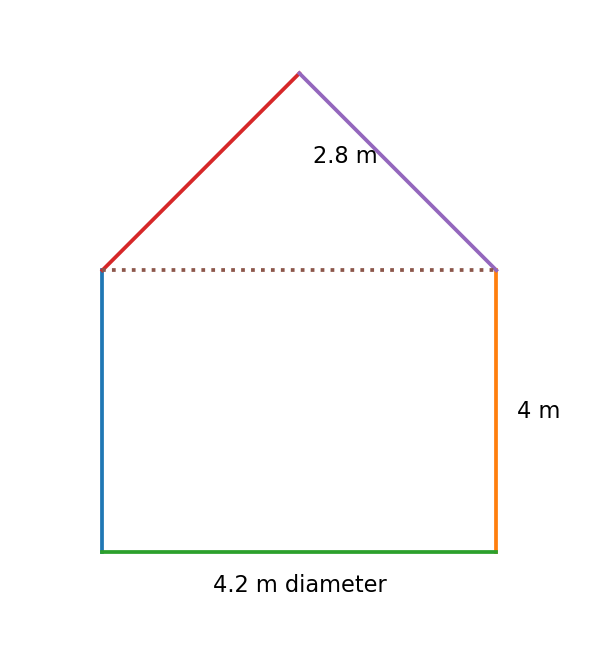
\includegraphics[width=0.72\linewidth]{figs/Tent.png}\caption{The tent consists of a cylinder and a cone and has no canvas floor.}\label{fig:tent}\end{figure}
\solution The radius is $r=2.1\,\mathrm m$. The cone's slant height is, by \eqref{eq:cone-formula},
\begin{equation}
\ell=\sqrt{2.1^2+2.8^2}=3.5\,\mathrm m.
\end{equation}
Only the curved cylinder and cone surfaces need canvas. Their combined area is
\begin{align}
A&=2\pi rh+\pi r\ell\\
&=2\pi(2.1)(4)+\pi(2.1)(3.5)=75.9\,\mathrm m^2.
\end{align}
For 100 tents, the total cost is $100\times75.9\times100=\text{Rs. }759{,}000$. Half is $\text{Rs. }379{,}500$. The plan also shows cooperation, initiative and care for people affected by floods.


The tent cross-section is generated by this script:
\par\smallskip
\noindent\textbf{Code reference -- plotting}
\par\noindent\fbox{\parbox{\dimexpr\linewidth-2\fboxsep-2\fboxrule\relax}{\centering\texttt{codes/Q17.py}}}
\par\smallskip
\end{enumerate}

\begin{enumerate}[label={},leftmargin=0pt,itemsep=9pt]
\setcounter{qcurrent}{22}\setcounter{equation}{0}
\item[\textbf{1.2.22}] Find the 60th term of the AP $8,10,12,\ldots$ and the sum of its last 10 terms.
\solution Here $a=8$ and $d=2$. By \eqref{eq:ap},
\begin{equation}
t_{60}=8+59(2)=126.
\end{equation}
The 51st term is $t_{51}=8+50(2)=108$. The last ten terms run from 108 to 126, so
\begin{equation}
S_{\mathrm{last\ 10}}=\frac{10}{2}(108+126)=1170.
\end{equation}



The 60th term and final-ten-term sum are checked by this script:
\par\smallskip
\noindent\textbf{Code reference -- numerical verification}
\par\noindent\fbox{\parbox{\dimexpr\linewidth-2\fboxsep-2\fboxrule\relax}{\centering\texttt{codes/Q22.py}}}
\par\smallskip
\setcounter{qcurrent}{23}\setcounter{equation}{0}
\item[\textbf{1.2.23}] A train travels 54 km at speed $x$ km/h and then 63 km at $(x+6)$ km/h. The total journey takes 3 hours. Find $x$.
\solution By \eqref{eq:speed-time},
\begin{equation}
\frac{54}{x}+\frac{63}{x+6}=3.
\end{equation}
Multiplying by $x(x+6)$ gives $54(x+6)+63x=3x(x+6)$, and hence
\begin{equation}
x^2-33x-108=0=(x-36)(x+3).
\end{equation}
Speed must be positive, so $x=36\,\mathrm{km/h}$.




\setcounter{qcurrent}{27}\setcounter{equation}{0}
\item[\textbf{1.2.27}] Point $A$ is 20 m above a lake. The angle of elevation of a cloud is $30^\circ$, while the angle of depression of its reflection in the lake is $60^\circ$. Find the distance from $A$ to the cloud.
\begin{figure}[H]\centering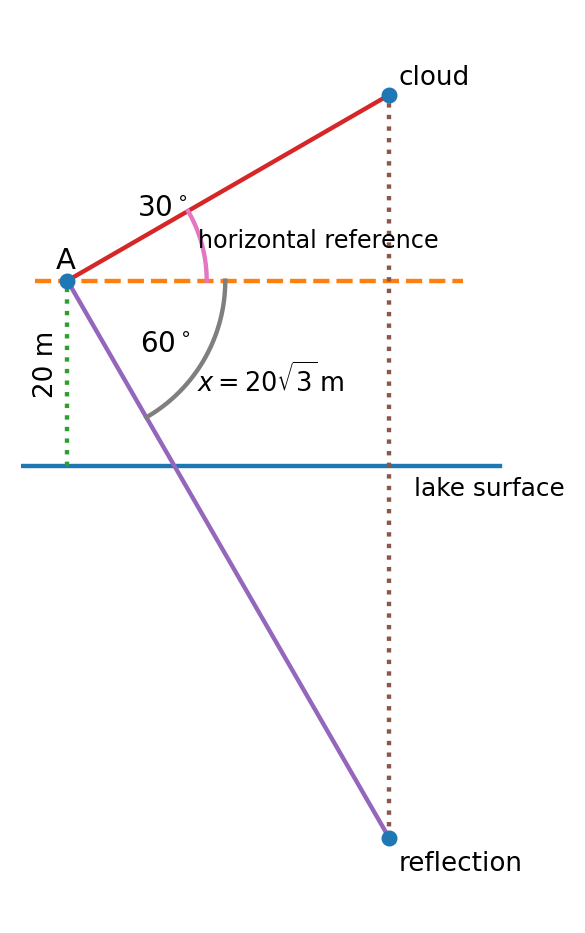
\includegraphics[height=0.42\textheight,keepaspectratio]{figs/CloudReflection.png}\caption{The reflection is as far below the lake surface as the cloud is above it.}\label{fig:cloud-reflection}\end{figure}
\solution Let $H$ be the cloud's height above the lake and let $x$ be the horizontal distance from $A$ to the vertical line through the cloud. The cloud is $H-20$ metres above $A$, while its reflection is $H+20$ metres below $A$. As shown in the figure, both the angle of elevation and the angle of depression are measured from the horizontal reference line through $A$. Using the two angles,
\begin{align}
\frac{H-20}{x}&=\tan30^\circ=\frac1{\sqrt3},\\
\frac{H+20}{x}&=\tan60^\circ=\sqrt3.
\end{align}
Rearranging produces a linear system in the unknowns $H$ and $x$:
\begin{equation}
\myvec{1&-1/\sqrt3\\1&-\sqrt3}\myvec{H\\x}=\myvec{20\\-20}.
\label{eq:q27system}
\end{equation}
For clarity, solve this system by Gaussian elimination. Its augmented matrix is
\begin{equation}
\left[\begin{array}{cc|c}1&-1/\sqrt3&20\\1&-\sqrt3&-20\end{array}\right]
\xrightarrow{\;R_2\leftarrow R_2-R_1\;}
\left[\begin{array}{cc|c}1&-1/\sqrt3&20\\0&-2/\sqrt3&-40\end{array}\right].
\end{equation}
The second row gives $-2x/\sqrt3=-40$, so $x=20\sqrt3\,\mathrm m$. Substitution into the first row yields $H-20=20$, so $H=40\,\mathrm m$. Hence the vertical separation between $A$ and the cloud is $H-20=20\,\mathrm m$. By Pythagoras,
\begin{equation}
AC=\sqrt{x^2+(H-20)^2}=\sqrt{(20\sqrt3)^2+20^2}=40\,\mathrm m.
\end{equation}



The linear system is solved independently and the angle diagram is generated by this script:
\par\smallskip
\noindent\textbf{Code reference -- plotting}
\par\noindent\fbox{\parbox{\dimexpr\linewidth-2\fboxsep-2\fboxrule\relax}{\centering\texttt{codes/Q27.py}}}
\par\smallskip
\setcounter{qcurrent}{28}\setcounter{equation}{0}
\item[\textbf{1.2.28}] A card is drawn from a well-shuffled 52-card deck. Find the probability that it is (i) a spade or an ace, (ii) a black king, (iii) neither a jack nor a king, (iv) either a king or a queen.
\solution Use \eqref{eq:prob-classical} and \eqref{eq:prob-union}:
\begin{enumerate}[label=(\roman*)]
\item The 13 spades and 4 aces overlap at the ace of spades. Thus $P=(13+4-1)/52=4/13$.
\item There are two black kings, so $P=2/52=1/26$.
\item There are four jacks and four kings. Their complement contains $52-4-4=44$ cards, so $P=44/52=11/13$.
\item Kings and queens are disjoint categories, each with four cards. Thus $P=(4+4)/52=2/13$.
\end{enumerate}

\setcounter{qcurrent}{29}\setcounter{equation}{0}
\item[\textbf{1.2.29}] Find $k$ if the triangle with vertices $(1,-1)$, $(-4,2k)$ and $(-k,-5)$ has area 24 square units.
\solution Taking differences of the coordinate vectors and using \eqref{eq:triangle-det},
\begin{equation}
2[ABC]=\left|\mydet{-5&2k+1\\-k-1&-4}\right|.
\end{equation}
Expanding the determinant gives
\begin{equation}
2[ABC]=|2k^2+3k+21|.
\end{equation}
Since $2k^2+3k+21$ has positive leading coefficient and discriminant $9-168=-159<0$, it is positive for every real $k$. The specified area is 24, so the determinant's absolute value is 48 and
\begin{equation}
2k^2+3k+21=48\quad\Longrightarrow\quad2k^2+3k-27=0.
\end{equation}
Applying the quadratic formula, the discriminant is $3^2-4(2)(-27)=225$, hence
\begin{equation}
k=\frac{-3\pm\sqrt{225}}4=\frac{-3\pm15}4.
\end{equation}
Therefore both solutions are valid: $k=3\quad\text{or}\quad k=-\frac92$.



\begin{figure}[H]\centering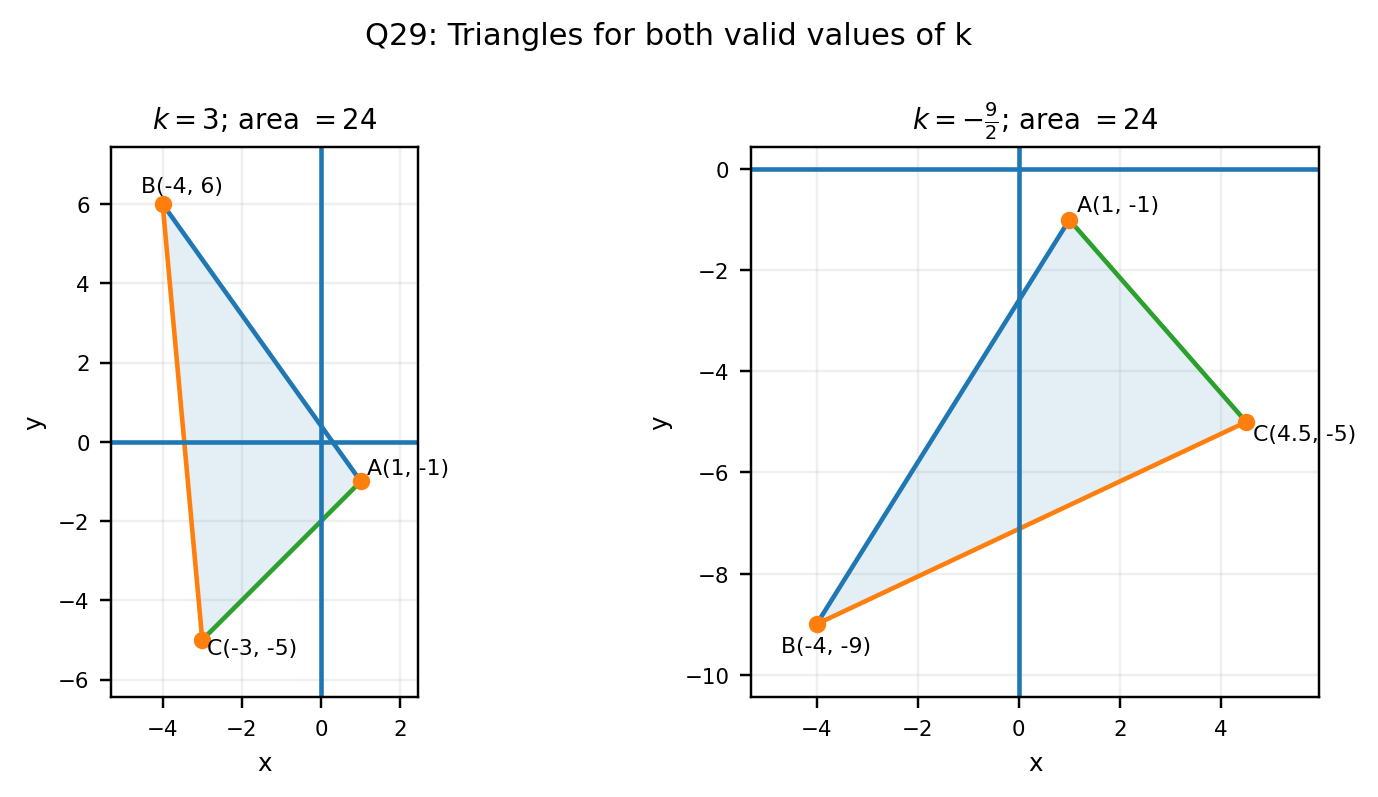
\includegraphics[width=0.99\linewidth]{figs/Q29_Triangles.png}\caption{The triangle formed by the given coordinates for each valid solution, $k=3$ and $k=-\frac92$. Both triangles have area 24 square units.}\label{fig:q29-triangles}\end{figure}
The Python code plots the triangles for the two theoretically derived values of $k$, using the CoordGeo triangle-area helper for the displayed areas:
\par\smallskip
\noindent\textbf{Code reference -- plotting}
\par\noindent\fbox{\parbox{\dimexpr\linewidth-2\fboxsep-2\fboxrule\relax}{\centering\texttt{codes/Q29.py}}}
\par\smallskip
\setcounter{qcurrent}{30}\setcounter{equation}{0}
\item[\textbf{1.2.30}] A square lawn has side 42 m. Two circular flower beds lie outside the vertical sides, with each circle centred at the intersection $O$ of the square's diagonals. Find the total shaded area. Use $\pi=22/7$.
\begin{figure}[H]\centering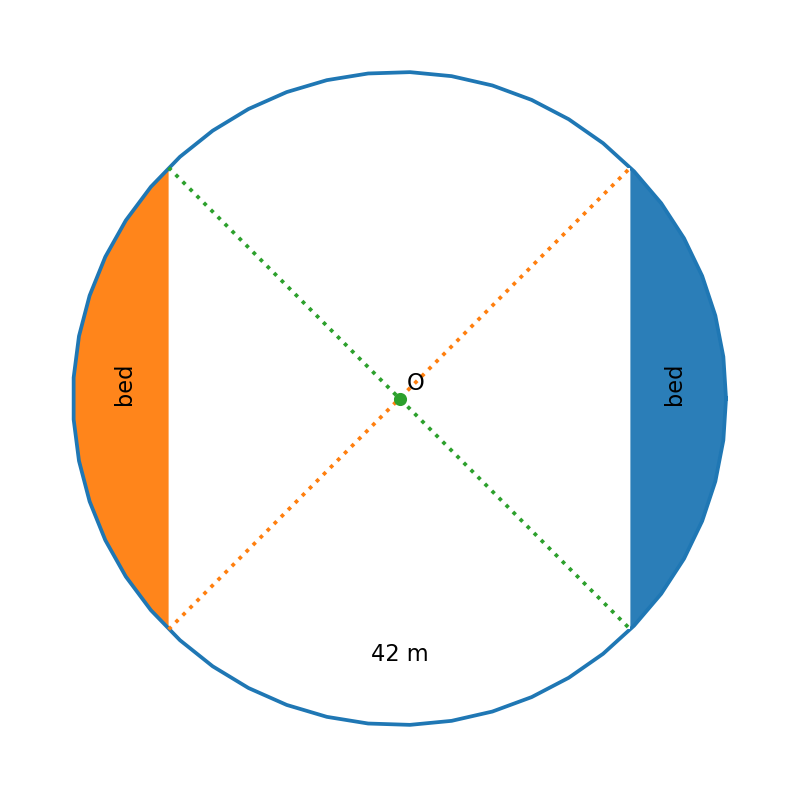
\includegraphics[width=0.84\linewidth]{figs/FlowerBeds.png}\caption{The shaded parts are the two circular segments outside the square lawn.}\label{fig:flower-beds}\end{figure}
\solution The radius from the centre to a corner is half the diagonal. Thus
\begin{equation}
r^2=\frac{42^2+42^2}{4}=882\,\mathrm{m}^2.
\end{equation}
Each vertical side subtends $90^\circ$ at $O$. The area of one segment is the area of a quarter-circle sector minus the right triangle with legs 21 m and 21 m:
\begin{equation}
A_1=\frac14\pi r^2-\frac12(42/2)^2=\frac{882\pi}{4}-441.
\end{equation}
The two beds are congruent, so
\begin{equation}
A_{\mathrm{total}}=2A_1=441\pi-882.
\end{equation}
Using $\pi=22/7$ gives $A_{\mathrm{total}}=1386-882=504\,\mathrm{m}^2$.



The flower-bed figure and shaded-area result are generated by this script:
\par\smallskip
\noindent\textbf{Code reference -- plotting}
\par\noindent\fbox{\parbox{\dimexpr\linewidth-2\fboxsep-2\fboxrule\relax}{\centering\texttt{codes/Q30.py}}}
\par\smallskip
\setcounter{qcurrent}{31}\setcounter{equation}{0}
\item[\textbf{1.2.31}] From both ends of a metal cylinder, hemispherical cavities of the same diameter are scooped out. The cylinder has height 10 cm and radius 4.2 cm. The remaining metal is made into a cylindrical wire of thickness 1.4 cm. Find the wire length. Use $\pi=22/7$.
\begin{figure}[H]\centering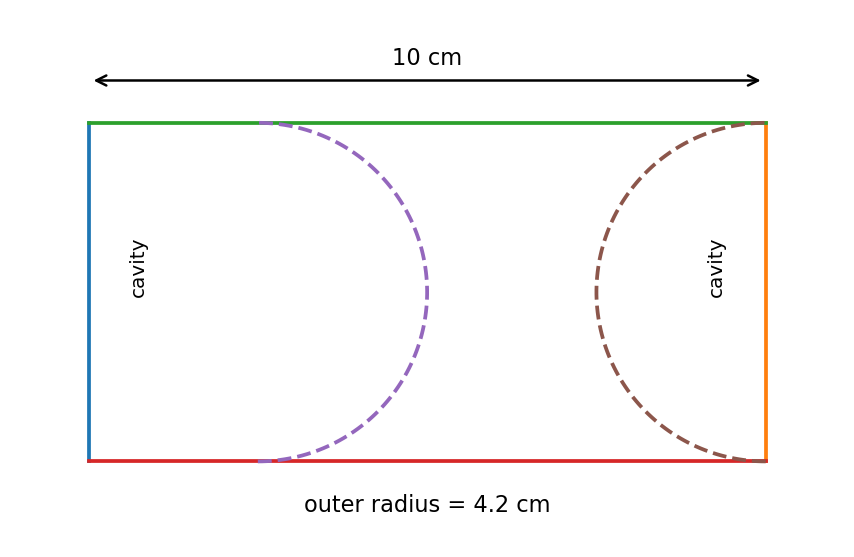
\includegraphics[width=0.84\linewidth]{figs/CylinderScooped.png}\caption{Two hemispherical cavities remove the volume of one sphere.}\label{fig:cylinder-scooped}\end{figure}
\solution The two hemispherical cavities together have the volume of one sphere. By \eqref{eq:scooped-cylinder}, the remaining metal has volume
\begin{equation}
V=\pi(4.2)^2(10)-\frac43\pi(4.2)^3=77.616\pi\,\mathrm{cm}^3.
\end{equation}
The wire's thickness is its diameter, so its radius is $0.7$ cm. Equating the volumes gives
\begin{equation}
\pi(0.7)^2L=77.616\pi\quad\Longrightarrow\quad L=\frac{77.616}{0.49}=158.4\,\mathrm{cm}.
\end{equation}


The cylinder-and-cavities diagram is generated by this script:
\par\smallskip
\noindent\textbf{Code reference -- plotting}
\par\noindent\fbox{\parbox{\dimexpr\linewidth-2\fboxsep-2\fboxrule\relax}{\centering\texttt{codes/Q31.py}}}
\par\smallskip
\end{enumerate}


\end{document}
